\section{Megvalósítás}
\subsection{Használt erőforrások}
A háló összerakást saját gépen kezdtük el. Majd a véglegesítését és a tanításokat AWS szerveren, NVIDIA Tesla K80 12GB videokártyán végeztük. Jupyter notebook-ban futtatuk a tanításokat, ezek elmentett adatait aztán Tensorboard segítségével elemeztük.

\subsection{Eredmények}

Zöngésség becslésére nagyon jó, alapfrekvencia (pitch érték) meghatározására használhatóan jó és a spektrális paraméter (Mel-Cepstrum) jósolására kezdetleges eredményeket sikerült elérnünk. (utóbbiról ezért nem is mellékeltünk tanítási és validációs grafikonokat). Hiperparaméter optimalizálás tekintetében egyelőre kézzel dolgoztunk (ez még javításra szorul), már így is sikerült használható pontosságot  elérnünk.

\textit{(A grafikonk y tengelyén az MSE hiba értéke x tengelyén az elvégzett epoch-ok száma látható.)}

\begin{minipage}{0.5\textwidth}
	Zöngésség becslése egyszerűbb, futásidő tekintetében gyorsabb feladatnak bizonyult. Ezért itt nem alkalmaztunk early stopping-ot, hanem a több próbálkozás után a fixen 410 epoch-kal történő tanításnál maradtunk.
	
	A teszt adatainkon elért eredmények:
	
	pontosság 0.8342
	
	költségfüggvény: 0.1560
	
	\textit{(MSE hiba értékekkel számítva)}
\end{minipage}
\begin{minipage}{0.5\textwidth}
	\flushright	
	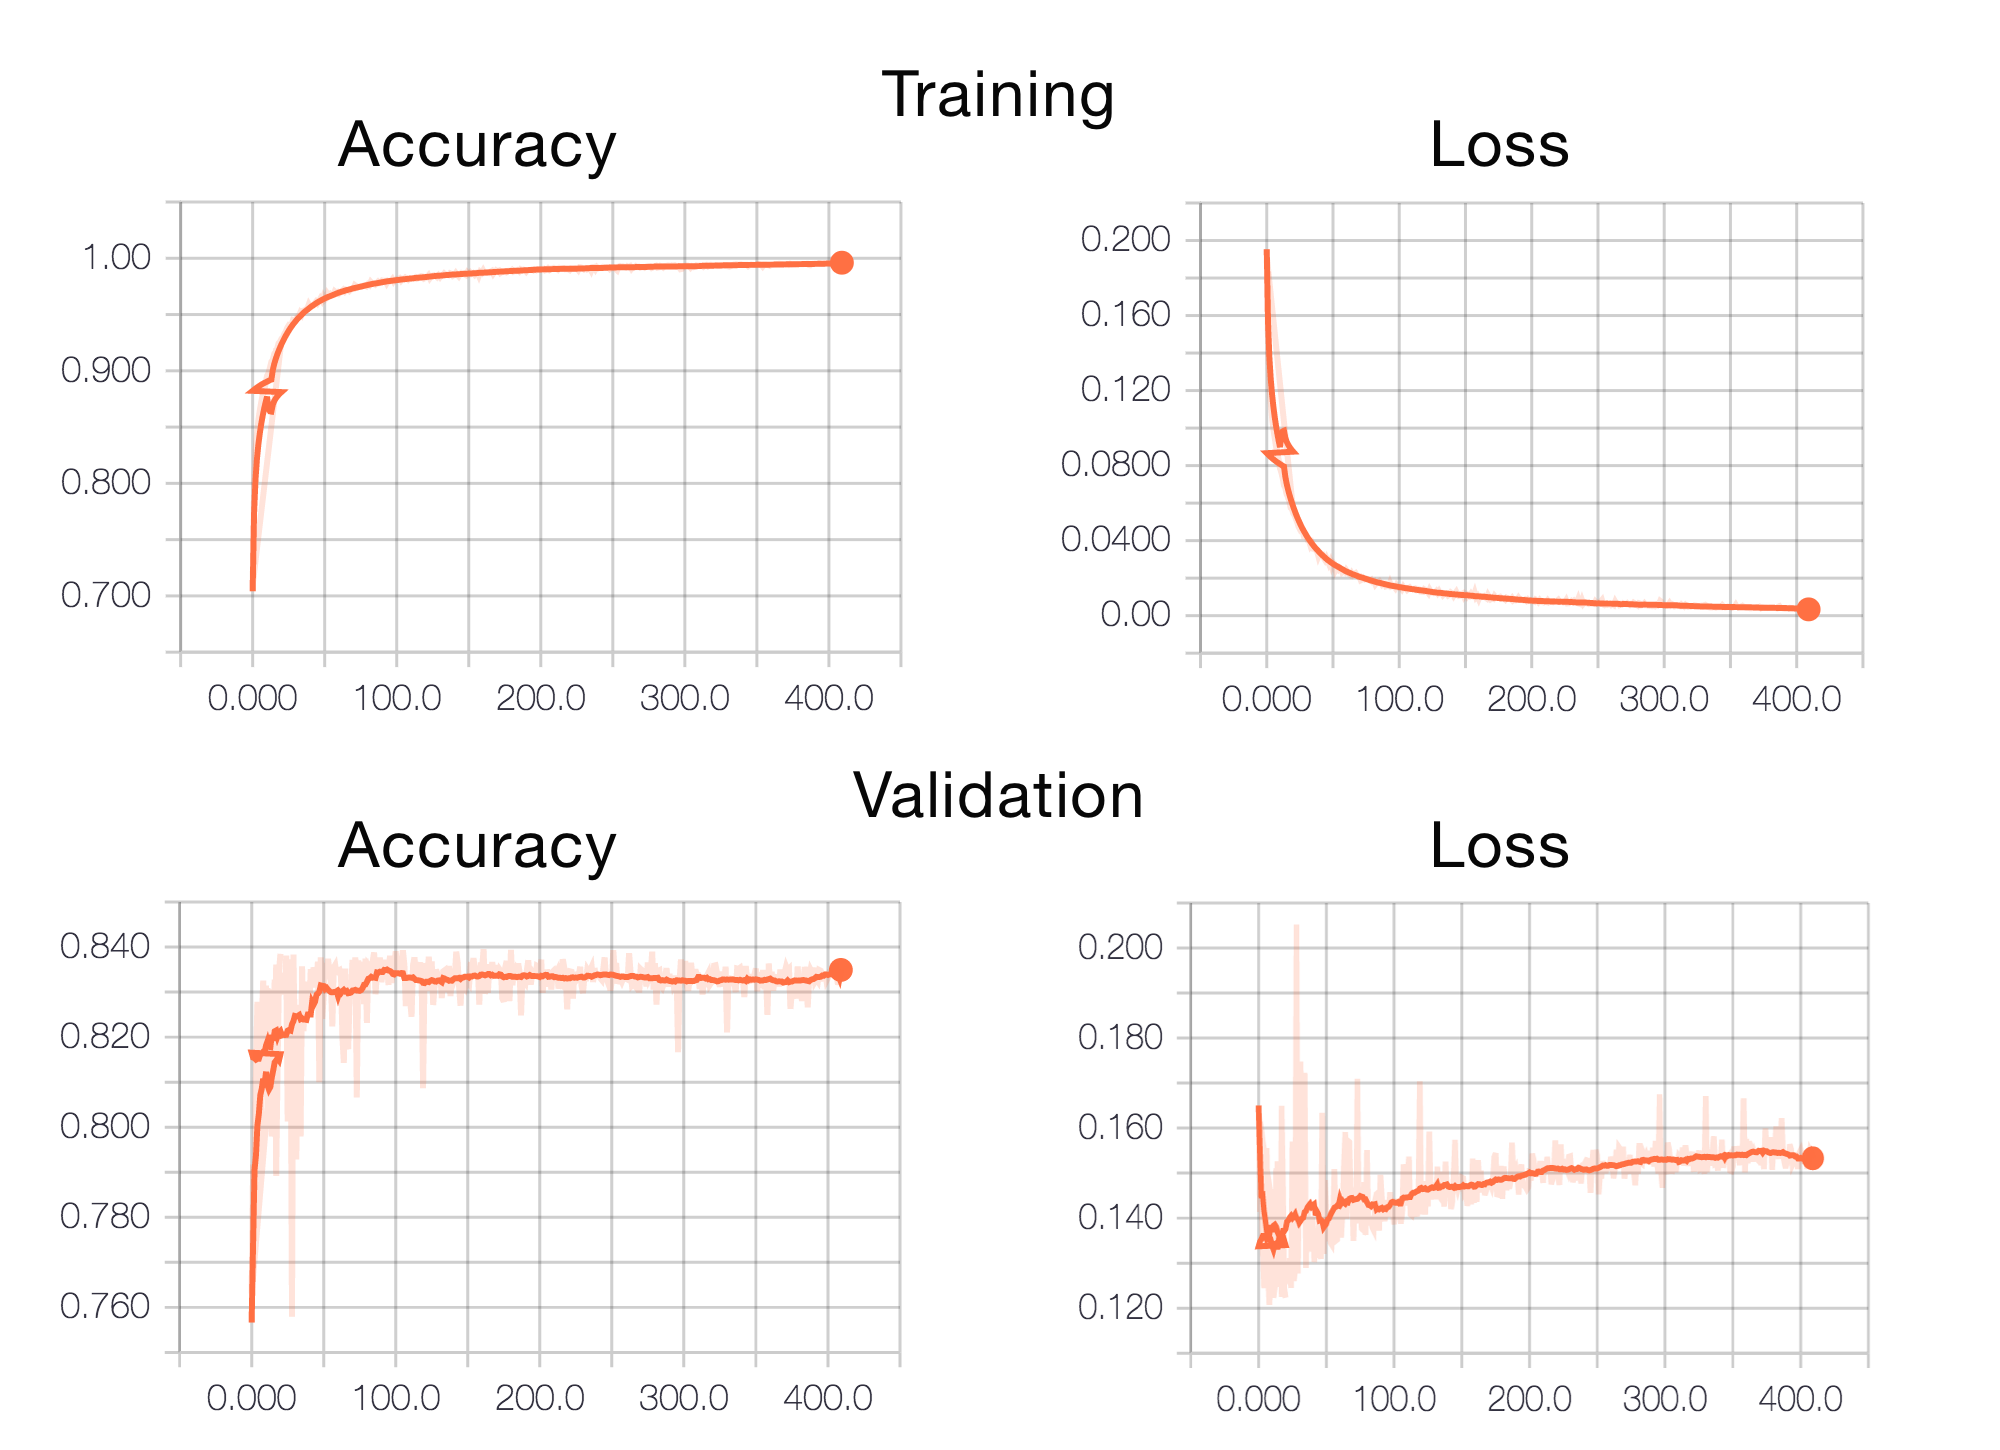
\includegraphics[width=0.8\textwidth,keepaspectratio]{uv_fig}
\end{minipage}

Az alapfrekvencia tanítása esetén alkalmaztunk early stoppig-ot. Ez azonban (a paramétereinek állítása után is) túl hamar állt meg. Ennek következtében több tanítást is elvégeztünk egymás után. Az itt kapott eredményeink messze nem olyan szépek mint a zöngésségé, de ezek is használhatónak bizonyultak.

A teszt adatainkon elért eredmények:

pontosság: 0.4243

költségfüggvény: 0.07214

\textit{(MSE hiba értékekkel számítva)}

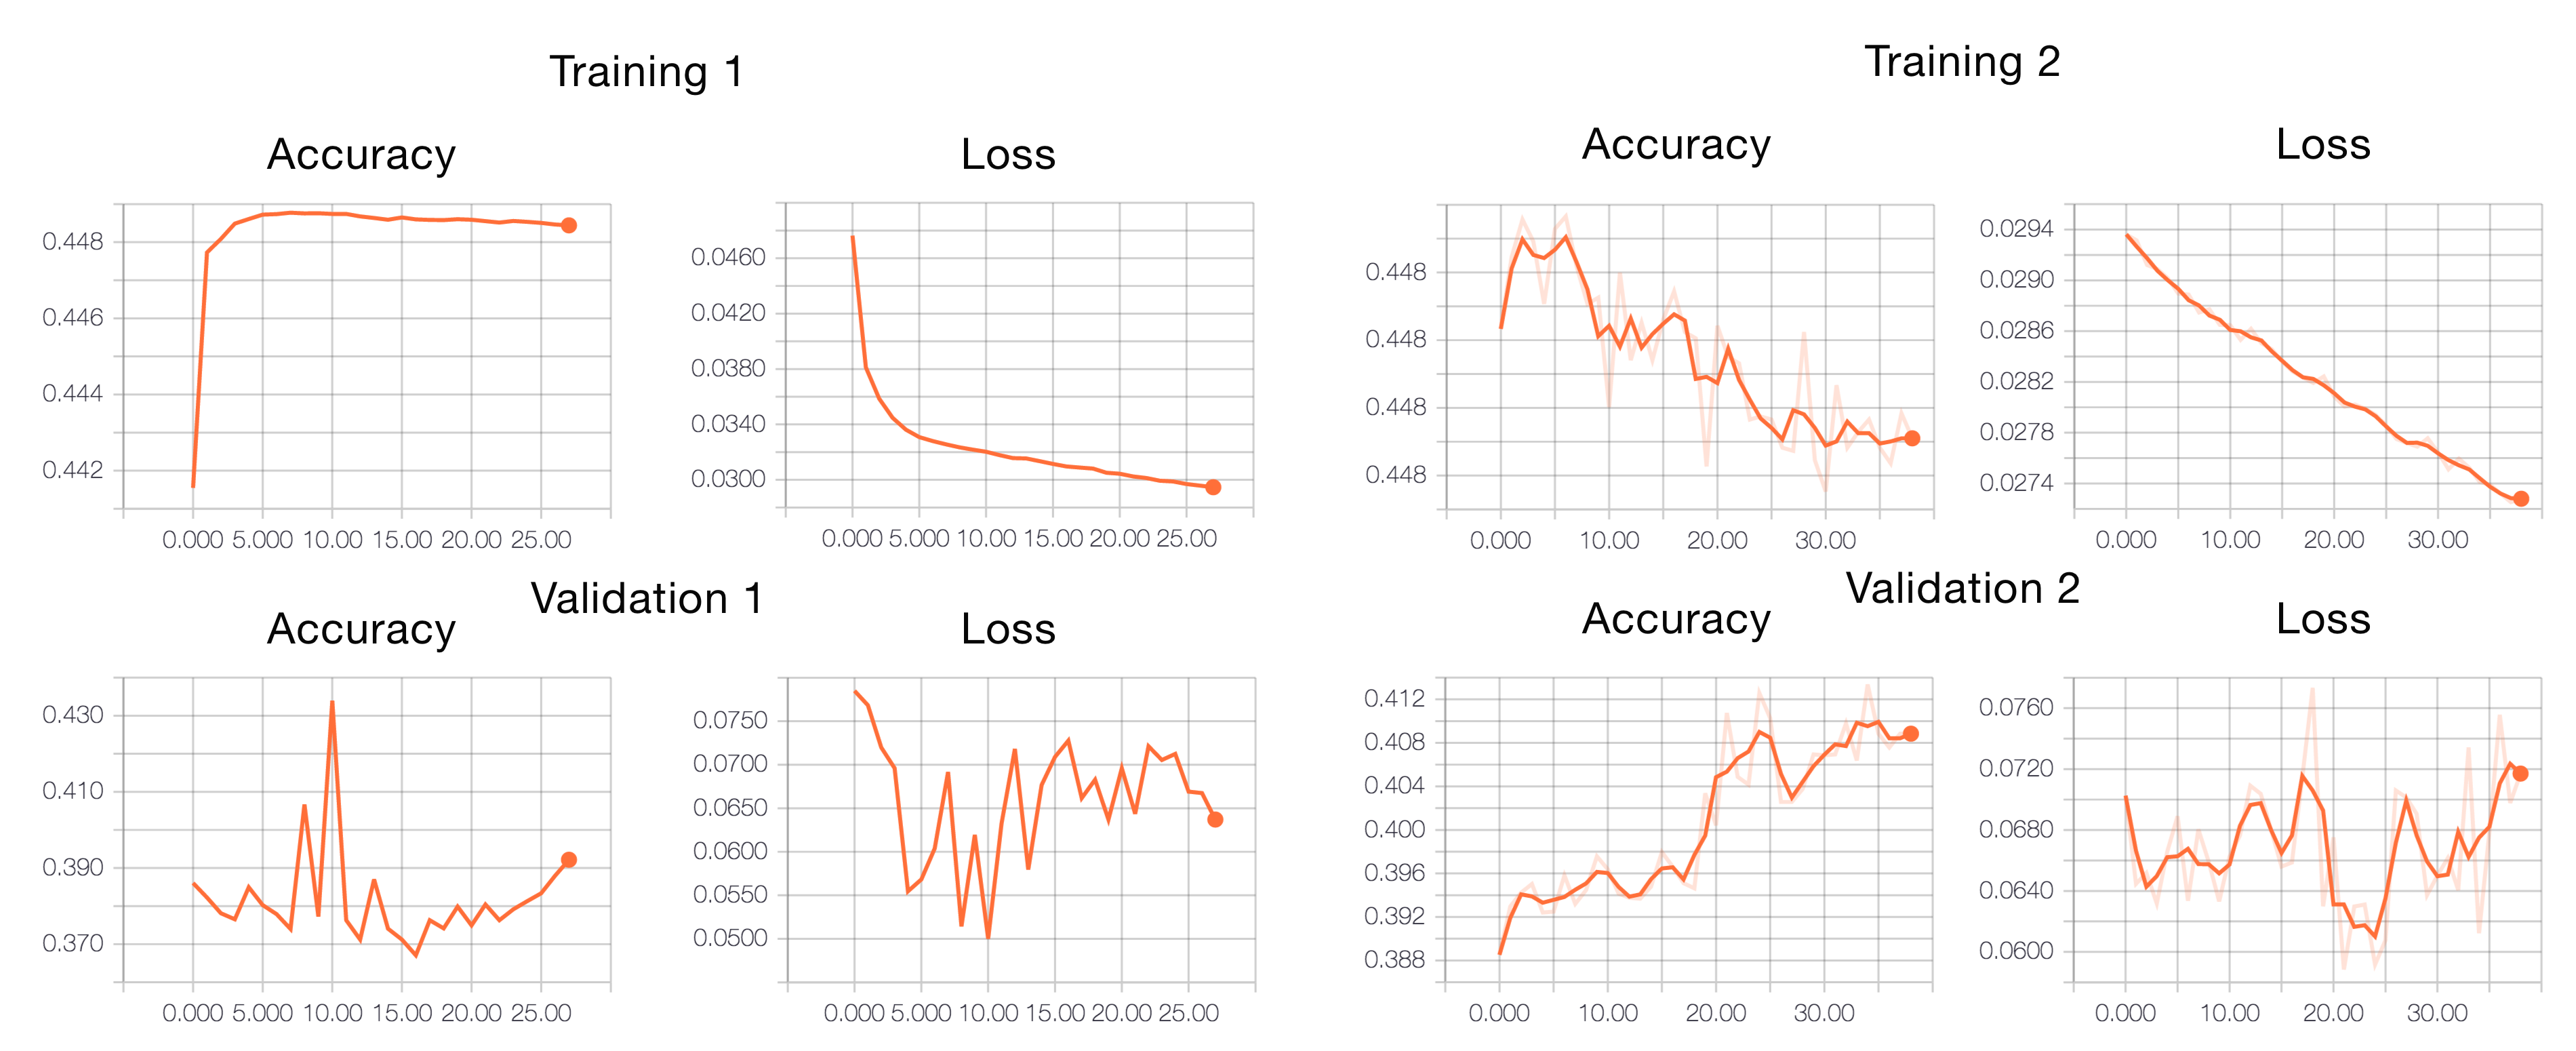
\includegraphics[width=\textwidth,keepaspectratio]{pitch_fig}